% Options for packages loaded elsewhere
\PassOptionsToPackage{unicode}{hyperref}
\PassOptionsToPackage{hyphens}{url}
%
\documentclass[
  english,
  man,floatsintext]{apa6}
\usepackage{amsmath,amssymb}
\usepackage{lmodern}
\usepackage{ifxetex,ifluatex}
\ifnum 0\ifxetex 1\fi\ifluatex 1\fi=0 % if pdftex
  \usepackage[T1]{fontenc}
  \usepackage[utf8]{inputenc}
  \usepackage{textcomp} % provide euro and other symbols
\else % if luatex or xetex
  \usepackage{unicode-math}
  \defaultfontfeatures{Scale=MatchLowercase}
  \defaultfontfeatures[\rmfamily]{Ligatures=TeX,Scale=1}
\fi
% Use upquote if available, for straight quotes in verbatim environments
\IfFileExists{upquote.sty}{\usepackage{upquote}}{}
\IfFileExists{microtype.sty}{% use microtype if available
  \usepackage[]{microtype}
  \UseMicrotypeSet[protrusion]{basicmath} % disable protrusion for tt fonts
}{}
\makeatletter
\@ifundefined{KOMAClassName}{% if non-KOMA class
  \IfFileExists{parskip.sty}{%
    \usepackage{parskip}
  }{% else
    \setlength{\parindent}{0pt}
    \setlength{\parskip}{6pt plus 2pt minus 1pt}}
}{% if KOMA class
  \KOMAoptions{parskip=half}}
\makeatother
\usepackage{xcolor}
\IfFileExists{xurl.sty}{\usepackage{xurl}}{} % add URL line breaks if available
\IfFileExists{bookmark.sty}{\usepackage{bookmark}}{\usepackage{hyperref}}
\hypersetup{
  pdftitle={Replication analysis of experiment 1, Coordinating bodies and mind. Behavioral synchrony fosters mentalizing},
  pdfauthor={Amanda Murphy1 \& Adam Baimel1,2},
  pdflang={en-EN},
  pdfkeywords={Interpersonal coordination,Mentalizing,Perspective taking,Mind, perception},
  hidelinks,
  pdfcreator={LaTeX via pandoc}}
\urlstyle{same} % disable monospaced font for URLs
\usepackage{graphicx}
\makeatletter
\def\maxwidth{\ifdim\Gin@nat@width>\linewidth\linewidth\else\Gin@nat@width\fi}
\def\maxheight{\ifdim\Gin@nat@height>\textheight\textheight\else\Gin@nat@height\fi}
\makeatother
% Scale images if necessary, so that they will not overflow the page
% margins by default, and it is still possible to overwrite the defaults
% using explicit options in \includegraphics[width, height, ...]{}
\setkeys{Gin}{width=\maxwidth,height=\maxheight,keepaspectratio}
% Set default figure placement to htbp
\makeatletter
\def\fps@figure{htbp}
\makeatother
\setlength{\emergencystretch}{3em} % prevent overfull lines
\providecommand{\tightlist}{%
  \setlength{\itemsep}{0pt}\setlength{\parskip}{0pt}}
\setcounter{secnumdepth}{-\maxdimen} % remove section numbering
% Make \paragraph and \subparagraph free-standing
\ifx\paragraph\undefined\else
  \let\oldparagraph\paragraph
  \renewcommand{\paragraph}[1]{\oldparagraph{#1}\mbox{}}
\fi
\ifx\subparagraph\undefined\else
  \let\oldsubparagraph\subparagraph
  \renewcommand{\subparagraph}[1]{\oldsubparagraph{#1}\mbox{}}
\fi
% Manuscript styling
\usepackage{upgreek}
\captionsetup{font=singlespacing,justification=justified}

% Table formatting
\usepackage{longtable}
\usepackage{lscape}
% \usepackage[counterclockwise]{rotating}   % Landscape page setup for large tables
\usepackage{multirow}		% Table styling
\usepackage{tabularx}		% Control Column width
\usepackage[flushleft]{threeparttable}	% Allows for three part tables with a specified notes section
\usepackage{threeparttablex}            % Lets threeparttable work with longtable

% Create new environments so endfloat can handle them
% \newenvironment{ltable}
%   {\begin{landscape}\centering\begin{threeparttable}}
%   {\end{threeparttable}\end{landscape}}
\newenvironment{lltable}{\begin{landscape}\centering\begin{ThreePartTable}}{\end{ThreePartTable}\end{landscape}}

% Enables adjusting longtable caption width to table width
% Solution found at http://golatex.de/longtable-mit-caption-so-breit-wie-die-tabelle-t15767.html
\makeatletter
\newcommand\LastLTentrywidth{1em}
\newlength\longtablewidth
\setlength{\longtablewidth}{1in}
\newcommand{\getlongtablewidth}{\begingroup \ifcsname LT@\roman{LT@tables}\endcsname \global\longtablewidth=0pt \renewcommand{\LT@entry}[2]{\global\advance\longtablewidth by ##2\relax\gdef\LastLTentrywidth{##2}}\@nameuse{LT@\roman{LT@tables}} \fi \endgroup}

% \setlength{\parindent}{0.5in}
% \setlength{\parskip}{0pt plus 0pt minus 0pt}

% \usepackage{etoolbox}
\makeatletter
\patchcmd{\HyOrg@maketitle}
  {\section{\normalfont\normalsize\abstractname}}
  {\section*{\normalfont\normalsize\abstractname}}
  {}{\typeout{Failed to patch abstract.}}
\patchcmd{\HyOrg@maketitle}
  {\section{\protect\normalfont{\@title}}}
  {\section*{\protect\normalfont{\@title}}}
  {}{\typeout{Failed to patch title.}}
\makeatother
\shorttitle{Title}
\keywords{Interpersonal coordination,Mentalizing,Perspective taking,Mind, perception\newline\indent Word count: X}
\usepackage{lineno}

\linenumbers
\usepackage{csquotes}
\ifxetex
  % Load polyglossia as late as possible: uses bidi with RTL langages (e.g. Hebrew, Arabic)
  \usepackage{polyglossia}
  \setmainlanguage[]{english}
\else
  \usepackage[main=english]{babel}
% get rid of language-specific shorthands (see #6817):
\let\LanguageShortHands\languageshorthands
\def\languageshorthands#1{}
\fi
\ifluatex
  \usepackage{selnolig}  % disable illegal ligatures
\fi
\newlength{\cslhangindent}
\setlength{\cslhangindent}{1.5em}
\newlength{\csllabelwidth}
\setlength{\csllabelwidth}{3em}
\newenvironment{CSLReferences}[2] % #1 hanging-ident, #2 entry spacing
 {% don't indent paragraphs
  \setlength{\parindent}{0pt}
  % turn on hanging indent if param 1 is 1
  \ifodd #1 \everypar{\setlength{\hangindent}{\cslhangindent}}\ignorespaces\fi
  % set entry spacing
  \ifnum #2 > 0
  \setlength{\parskip}{#2\baselineskip}
  \fi
 }%
 {}
\usepackage{calc}
\newcommand{\CSLBlock}[1]{#1\hfill\break}
\newcommand{\CSLLeftMargin}[1]{\parbox[t]{\csllabelwidth}{#1}}
\newcommand{\CSLRightInline}[1]{\parbox[t]{\linewidth - \csllabelwidth}{#1}\break}
\newcommand{\CSLIndent}[1]{\hspace{\cslhangindent}#1}

\title{Replication analysis of experiment 1, Coordinating bodies and mind. Behavioral synchrony fosters mentalizing}
\author{Amanda Murphy\textsuperscript{1} \& Adam Baimel\textsuperscript{1,2}}
\date{}


\affiliation{\vspace{0.5cm}\textsuperscript{1} Brooklyn College CUNY\\\textsuperscript{2} The University of British Columbia}

\abstract{
The study was condutcted by : Baimel, Birch, S. A. ., \& Norenzayan, A. 2018. The original paper can be retrieved from \url{https://doi.org/10.1016/j.jesp.2017.10.008})

The practice of collective rituals using synchronized group movements has been around for centuries. Anthropologists have referenced group practices as being a major component in relating the self to others, as well as fostering social cohesion and cooperation.

`Attentional focus on others' while in a collective practice questions if there is a simultaneous perception of others' actions and if this may involve the same neural pathways in the perceiver when being in sync with others. Further, the bridge between others and self in physical movements has been thought to influence a greater perspective taking of the other and therefore a higher ability in empaphizing.

The study of comparing in-time synchronized movements with others in comparison to the same movements at different times than the group has is a main focus for researchers in experiment 1 of this study. This condition, asynchronous and synchronous body movements was compared with the likeliness of taking the perspective of others in the form of an empathy quotient questionnaire.

In experiment one, synchronous movements as opposed to asynchronous movements, increased self reported results in the tendency and ability for considering other's mental states as shown by results in the empathy quotient.
}



\begin{document}
\maketitle

\hypertarget{methods}{%
\section{Methods}\label{methods}}

The self report `Empathy Quotient' was used to measure if individuals in general considered other's mental states. The dependent variable was measured by a synchronized participation task. More specifically, whether or not individuals were assigned to move synchronously or asynchronously to a musical performance task. Data for experiment 1 used in this replication can be found at:
\url{https://osf.io/5d4f6/}

\hypertarget{participants}{%
\subsection{Participants}\label{participants}}

N= 116

\hypertarget{procedure}{%
\subsection{Procedure}\label{procedure}}

\hypertarget{data-analysis}{%
\subsection{Data analysis}\label{data-analysis}}

We used R {[}Version 4.1.1; R Core Team (2021){]} and the R-packages \emph{data.table} {[}Version 1.14.0; Dowle and Srinivasan (2021){]}, \emph{dplyr} {[}Version 1.0.7; Wickham, François, Henry, and Müller (2021){]}, \emph{ggplot2} {[}Version 3.3.5; Wickham (2016){]}, \emph{papaja} {[}Version 0.1.0.9997; Aust and Barth (2020){]}, and \emph{readr} {[}Version 2.0.1; Wickham and Hester (2021){]} for all our analyses.

\begin{verbatim}
## $estimate
## [1] "$\\Delta M = -3.79$, 95\\% CI $[-7.54$, $-0.04]$"
## 
## $statistic
## [1] "$t(114) = -2.00$, $p = .048$"
## 
## $full_result
## [1] "$\\Delta M = -3.79$, 95\\% CI $[-7.54$, $-0.04]$, $t(114) = -2.00$, $p = .048$"
## 
## $table
## NULL
## 
## attr(,"class")
## [1] "apa_results" "list"
\end{verbatim}

\hypertarget{results}{%
\section{Results}\label{results}}

The reanalysis for the async and sync conditions for the empathy quotient were significant in showing that those who performed synchronous movements as part of the experiment rated higher in taking others perspectives in to consideration as measured by the empathy quotient. \(\Delta M = -3.79\), 95\% CI \([-7.54\), \(-0.04]\), \(t(114) = -2.00\), \(p = .048\), \(\Delta M = -3.79\), 95\% CI \([-7.54\), \(-0.04]\), \(t(114) = -2.00\), \(p = .048\), NULL

\begin{tabular}{l|r}
\hline
condition & means\\
\hline
async & 42.20968\\
\hline
sync & 46.00000\\
\hline
\end{tabular}

\begin{figure}
\centering
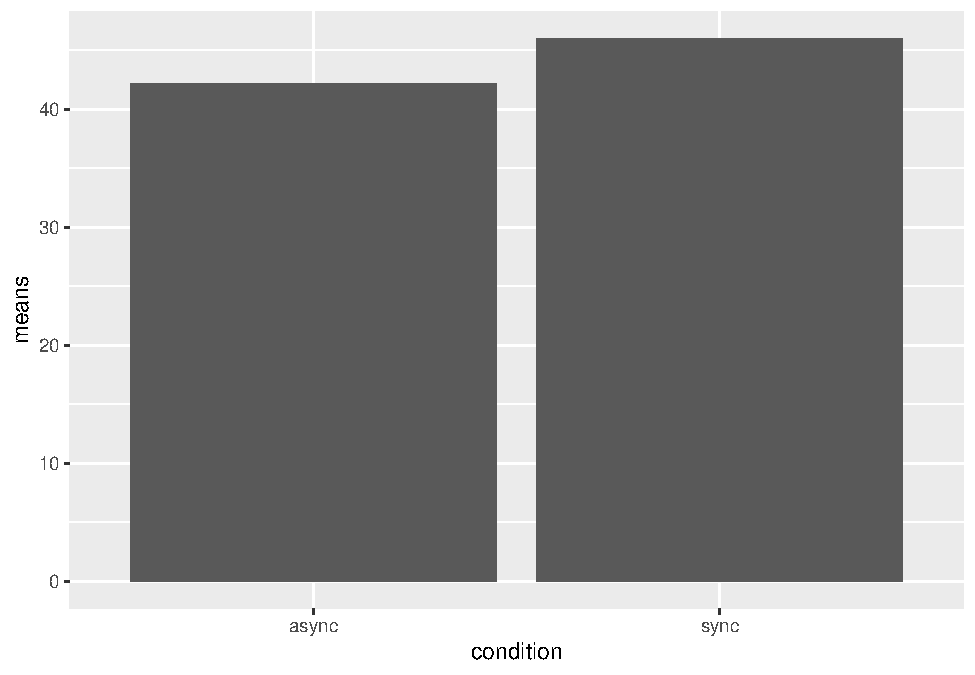
\includegraphics{Manuscript.final_files/figure-latex/unnamed-chunk-3-1.pdf}
\caption{\label{fig:unnamed-chunk-3}Means of empathy quotient scores in Sync and Async groups.}
\end{figure}

\newpage

\#Power Analysis

The following reports a power analysis for the t-test used in experiment 1.This shows the power of this design to detect the effect size at different sample sizes.

\begin{figure}
\centering
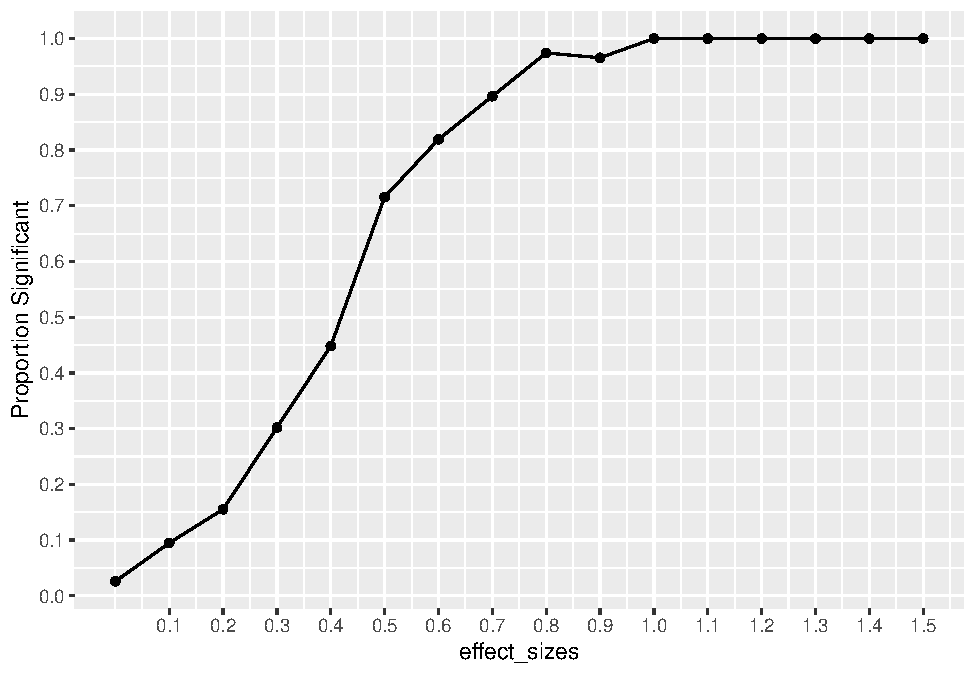
\includegraphics{Manuscript.final_files/figure-latex/unnamed-chunk-4-1.pdf}
\caption{\label{fig:unnamed-chunk-4}A power curve analysis for an independent t-test with 116 participants.}
\end{figure}

\hypertarget{discussion}{%
\section{Discussion}\label{discussion}}

The re-analysis successfully reproduced the analysis reported by Baimel, Birch, and Norenzayan (2018).

\hypertarget{references}{%
\section{References}\label{references}}

\begingroup
\setlength{\parindent}{-0.5in}
\setlength{\leftskip}{0.5in}

\hypertarget{refs}{}
\begin{CSLReferences}{1}{0}
\leavevmode\hypertarget{ref-R-papaja}{}%
Aust, F., \& Barth, M. (2020). \emph{{papaja}: {Create} {APA} manuscripts with {R Markdown}}. Retrieved from \url{https://github.com/crsh/papaja}

\leavevmode\hypertarget{ref-baimel2018coordinating}{}%
Baimel, A., Birch, S. A., \& Norenzayan, A. (2018). Coordinating bodies and minds: Behavioral synchrony fosters mentalizing. \emph{Journal of Experimental Social Psychology}, \emph{74}, 281--290.

\leavevmode\hypertarget{ref-R-data.table}{}%
Dowle, M., \& Srinivasan, A. (2021). \emph{Data.table: Extension of `data.frame`}. Retrieved from \url{https://CRAN.R-project.org/package=data.table}

\leavevmode\hypertarget{ref-R-base}{}%
R Core Team. (2021). \emph{R: A language and environment for statistical computing}. Vienna, Austria: R Foundation for Statistical Computing. Retrieved from \url{https://www.R-project.org/}

\leavevmode\hypertarget{ref-R-ggplot2}{}%
Wickham, H. (2016). \emph{ggplot2: Elegant graphics for data analysis}. Springer-Verlag New York. Retrieved from \url{https://ggplot2.tidyverse.org}

\leavevmode\hypertarget{ref-R-dplyr}{}%
Wickham, H., François, R., Henry, L., \& Müller, K. (2021). \emph{Dplyr: A grammar of data manipulation}. Retrieved from \url{https://CRAN.R-project.org/package=dplyr}

\leavevmode\hypertarget{ref-R-readr}{}%
Wickham, H., \& Hester, J. (2021). \emph{Readr: Read rectangular text data}. Retrieved from \url{https://CRAN.R-project.org/package=readr}

\end{CSLReferences}

\endgroup


\end{document}
